\documentclass[11pt]{article}
\usepackage[T1]{fontenc}
\usepackage[utf8]{inputenc}
\usepackage[a4paper,margin=25mm]{geometry}
\usepackage{amsmath,amssymb,amsthm}
\usepackage{tikz}
\usetikzlibrary{calc,positioning,arrows.meta}
\usepackage{hyperref,xurl}
\newtheorem{theorem}{Theorem}
\newtheorem{lemma}[theorem]{Lemma}
\newtheorem{proposition}[theorem]{Proposition}
\newtheorem{corollary}[theorem]{Corollary}
\theoremstyle{remark}
\newtheorem{remark}[theorem]{Remark}
\newcommand{\HH}{\mathbb H}
\newcommand{\ip}[2]{\langle #1,#2\rangle}
\newcommand{\Vol}{\operatorname{Vol}}
\title{Perpendicular edges and facet capacity\linebreak
in compact right-angled hyperbolic four-polytopes}
\author{Coxeter Polytopes Frontier Project}
\date{18 October 2026}
\begin{document}
\maketitle

\begin{abstract}
If a facet of a compact right-angled hyperbolic four-polytope has $V$
vertices, the polytope has at least $2V+5$ facets. The proof counts the
opposite endpoints of edges perpendicular to a chosen facet, then uses
an ear argument to control the remaining facets. Equality in the
three-dimensional local count has the combinatorics of a L\"obell
polyhedron; the disjointness of its opposite face supplies the needed
four-dimensional capacity estimate. Together with the exact pentagon
excess identity, the result shows that a polytope of volume strictly
below that of the right-angled $120$-cell must have at most $48$ vertices
in every facet. It does not establish the $120$-cell minimum or a second
volume gap.
\end{abstract}

\section{Statement and scope}

Throughout, a polytope is convex and full-dimensional. A right-angled
hyperbolic polytope has dihedral angle $\pi/2$ at every ridge. All
polytopes in this paper are compact. In particular every edge has two
finite endpoints, and every two-face is a compact right-angled polygon.
If $P\subset\HH^4$, write $(v,e,r,f)$ for its numbers of vertices,
edges, ridges and facets.

\begin{theorem}\label{thm:capacity}
Let $F$ be a facet of a compact right-angled hyperbolic four-polytope
$P$. If $F$ has $V$ vertices, then
\begin{equation}\label{eq:capacity}
 f\ge 2V+5.
\end{equation}
\end{theorem}

Define the pentagon excess by
\[
 W=\sum_{R\text{ a ridge of }P}\bigl(k(R)-5\bigr),
\]
where $k(R)$ is the number of sides of $R$. We will prove
\begin{equation}\label{eq:volume}
 W=v-5f,\qquad
 \Vol(P)=\frac{\pi^2}{12}(f+W+16).
\end{equation}
For a facet $F$, put
\[
 d(F)=\sum_{R\subset F}\bigl(k(R)-5\bigr).
\]
If it has $V$ vertices, then $d(F)=(V-20)/2$ and $W\ge d(F)$.

\begin{corollary}\label{cor:local-size}
For every facet $F$ of $P$ with $V$ vertices,
\begin{equation}\label{eq:excess-bound}
 f+W\ge\frac52V-5.
\end{equation}
Consequently:
\begin{enumerate}
\item if $\Vol(P)<34\pi^2/3$, then every facet has at most $48$ vertices;
\item if $\Vol(P)\le34\pi^2/3$, then every facet has at most $50$ vertices;
\item if $\Vol(P)<68\pi^2/3$, then every facet has at most $104$ vertices.
\end{enumerate}
\end{corollary}

The comparison values are respectively the volume of the regular compact
right-angled $120$-cell and of its facet double. The corollary is a local
size reduction. No assertion about minimality, a second volume, or
decomposition into regular $120$-cells follows from it.

The geometric input is the usual acute-chamber wall property: distinct
outward unit normals of an acute-angled hyperbolic polytope have
nonpositive scalar products. We use the standard Lorentz model and the
ordinary dual cell decomposition of the boundary of a simple convex
polytope. These are the acute-angle facts discussed in
\cite[pp.~63--64 and Proposition~4.1]{PV}, with the general geometric
background in~\cite{AVS}. We prove below the stronger compact normal gap,
the intersection and distinctness statements used in the count, and the
needed planar closing argument. The volume discussion also uses
Chern--Gauss--Bonnet for a compact hyperbolic reflection orbifold; its
resulting face formula agrees with~\cite[Proposition~3.5(d)]{KP}. No
classification of compact right-angled three- or four-polytopes is an
input. In particular we do not assume uniqueness of a small facet or a
minimum-volume theorem.

\section{Normal geometry and perpendicular edges}

Use the hyperboloid model in $\mathbb R^{n,1}$, with scalar product of
signature $(-,+,\ldots,+)$. A point of $\HH^n$ is a future unit timelike
vector. An outward unit spacelike normal $a$ defines the half-space
$\ip{x}{a}\le0$.

\begin{lemma}\label{lem:gap}
Distinct wall normals of a compact right-angled polytope have product
either $0$ or strictly less than $-1$. A mutually orthogonal collection
of wall normals determines an actual common face.
\end{lemma}
\begin{proof}
Products are nonpositive by the acute-chamber wall property. Suppose
two normals $a,b$ have $g=\ip{a}{b}\in(-1,0)$. Their Gram matrix
\[
 G=\begin{pmatrix}1&g\\g&1\end{pmatrix}
\]
is positive definite and $G^{-1}$ has nonnegative entries. Let $p$ be a
strict future timelike interior point and set
$\beta=(\ip{p}{a},\ip{p}{b})^T<0$. The orthogonal projection
\[
 u=p-[a\ b]G^{-1}\beta
\]
adds nonnegative multiples of the outward normals to $p$. Thus it
strictly satisfies every other wall inequality. It satisfies the two
selected equalities, and
\[
 u^2=p^2-\beta^TG^{-1}\beta<0,\qquad
 \ip{p}{u}=u^2<0.
\]
It is therefore future timelike and gives an actual ridge, whose angle
is not $\pi/2$, a contradiction.

If $\ip{a}{b}=-1$, the nonzero vector $a+b$ is null. It has negative
product with $p$, hence is future. Its products with all other wall
normals are nonpositive. It would be a feasible ideal point, contrary
to compactness. The sum cannot be zero, because $p$ has negative product
with both summands. This proves the gap.

For mutually orthogonal normals $a_1,\ldots,a_j$, the same projection is
particularly simple:
\[
 u=p-\sum_{i=1}^j\ip{p}{a_i}a_i.
\]
It is future timelike, has zero product with each selected normal and
strict negative product with every other wall normal. Hence their
intersection is an actual codimension-$j$ face.
\end{proof}

At any finite vertex, all its incident normals lie in a positive definite
space. Lemma~\ref{lem:gap} makes them mutually orthogonal. There are
exactly $n$ of them, so the polytope is simple. A facet inherits right
angles: its neighboring wall normals are orthogonal to its own normal,
and serve as its intrinsic outward normals. The same applies to faces
of lower dimension. A compact right-angled $k$-gon has area
$(k-4)\pi/2>0$, so $k\ge5$.

\begin{lemma}\label{lem:footprint}
Fix a facet $A$ with normal $a$, and a facet disjoint from $A$ with
normal $z$. Any two common neighbors of these facets meet each other.
\end{lemma}
\begin{proof}
We have $\ip{a}{z}<-1$. The plane spanned by $a,z$ is Lorentzian, so
its orthogonal complement is positive definite. The normals $b,c$ of
two common neighbors belong to this complement. In a positive definite
space their product cannot be below $-1$. Product $-1$ would imply
$b=-c$, incompatible with a strict point of both negative half-spaces.
Lemma~\ref{lem:gap} therefore gives $\ip{b}{c}=0$, and the facets meet.
\end{proof}

We call the set of neighbors of $A$ meeting another facet its
\emph{footprint on the neighbors of $A$}. Lemma~\ref{lem:footprint}
says that a disjoint facet's footprint is a clique. This is the only
meaning of footprint used below.

\begin{lemma}\label{lem:opposite}
Let $A$ be a facet of a compact right-angled polytope in dimension three
or four. For every vertex $x$ of $A$, the edge leaving $A$ is perpendicular
to $A$ and ends on a facet $R_x$ disjoint from $A$. All the $R_x$ are
distinct. Moreover, $R_x$ meets a neighbor $B$ of $A$ if and only if $x$
belongs to $B$.

An actual facet disjoint from $A$ meeting all the neighbors of $A$ at
$x$ must be $R_x$.
\end{lemma}
\begin{proof}
Let $a$ be the outward normal of $A$. Regard $x$ as a vector in
$a^\perp$. Simplicity gives exactly one edge at $x$ not contained in
$A$. All its other defining walls are orthogonal to $a$, so its initial
direction is $-a$. If its length is $L_x>0$, the other endpoint is
\[
 y=\cosh(L_x)x-\sinh(L_x)a.
\]
The new normal there is forced to be
\begin{equation}\label{eq:opposite-normal}
 r_x=\sinh(L_x)x-\cosh(L_x)a.
\end{equation}
It is orthogonal to the walls defining the edge, has norm one and
satisfies $\ip{y}{r_x}=0$, $\ip{x}{r_x}<0$. Its product with $a$ is
$-\cosh(L_x)<-1$, so $R_x$ is disjoint from $A$.

For a neighbor $B$ with normal $b$,
\[
 \ip{r_x}{b}=\sinh(L_x)\ip{x}{b}.
\]
This is zero exactly when $x\in B$; the actual-intersection part of
Lemma~\ref{lem:gap} gives the stated incidence equivalence. If $r_x=r_y$,
projection to $a^\perp$ gives
$\sinh(L_x)x=\sinh(L_y)y$, hence $x=y$.

Finally a normal orthogonal to all the neighbors defining $x$ lies in
$\operatorname{span}(x,a)$. For an actual facet disjoint from $A$ its
orientation and its product with $x$ give the form
$r=\sinh(L)x-\cosh(L)a$, with $L>0$. Two distinct normals of this form
have product $\cosh(L-L_x)>0$, contrary to acuteness. Thus $r=r_x$.
\end{proof}

The final assertion is useful: a more distant wall on the same
perpendicular line cannot be counted as a second actual facet.

\section{Closing the neighborhood of a polygon}

\begin{lemma}\label{lem:polygon}
Let $Q\subset\HH^3$ be compact and right-angled, and let $A$ be a
$k$-gonal face. Then $Q$ has at least $2k+2$ faces. If it has exactly
$2k+2$, the unique face left after counting $A$, its $k$ neighbors and
its $k$ perpendicular-edge opposites is disjoint from all $k$ neighbors
of $A$.
\end{lemma}

\begin{proof}
Label the neighbors $A_1,\ldots,A_k$ cyclically. At the vertex where
$A_i$ and $A_{i+1}$ meet $A$, let $B_i$ be the opposite face supplied by
Lemma~\ref{lem:opposite}. Indices are cyclic. These are $1+2k$ distinct
faces. Among the $A_j$, the only neighbors of $B_i$ are $A_i,A_{i+1}$.
The $A_j$ themselves have just their cyclic adjacencies: any other
adjacency, together with $A$, would give an actual vertex of $A$ by
Lemma~\ref{lem:gap}.

Call any further face extra. Such a face meets at most one $A_i$.
Indeed two nonconsecutive $A_i$ cannot both meet it by
Lemma~\ref{lem:footprint}; meeting two consecutive ones would force it
to be the already counted $B_i$, by Lemma~\ref{lem:opposite}.

Pass to the dual triangulated two-sphere. Every vertex has degree at
least five, since every face of $Q$ is a compact right-angled polygon.
We use the elementary ear fact: a triangulated polygon with no interior
vertices has a vertex of degree two within that polygon. If one boundary
edge is prescribed, such an ear can be chosen away from its endpoints.
For example, root the tree dual to its triangles at that edge and take
a leaf away from the root; for a single triangle take the third vertex.

Suppose first there is no extra face. Each $A_i$ has exactly the five
known neighbors
\[
 A,\ A_{i-1},\ A_{i+1},\ B_{i-1},\ B_i.
\]
The cyclic link of $A_i$ forces the edge $B_{i-1}B_i$. The triangles
around $A$ and the $A_i$ form a disc whose complementary disc has boundary
$B_1,\ldots,B_k$ and no interior vertices. An ear in this disc has
degree two there, and has only its two outside neighbors $A_i,A_{i+1}$.
Its total degree would be four, a contradiction.

Now suppose there is exactly one extra face $C$, and it meets $A_i$.
It meets no other $A_j$. The five-neighbor argument still forces
$B_{j-1}B_j$ for $j\ne i$. At $A_i$ its cyclic link instead has the
segment $B_{i-1},C,B_i$. The complementary disc is therefore a polygon
with $C$ inserted into the $B$-cycle, again without interior vertices.
Every $B_j$ has just two outside $A$-neighbors, so needs degree at least
three within this disc. The vertex $C$ has just the outside neighbor
$A_i$, so needs degree at least four there. An ear is impossible. Hence
the unique extra face meets none of the $A_j$, as asserted.
\end{proof}

\begin{figure}[tb]
\centering
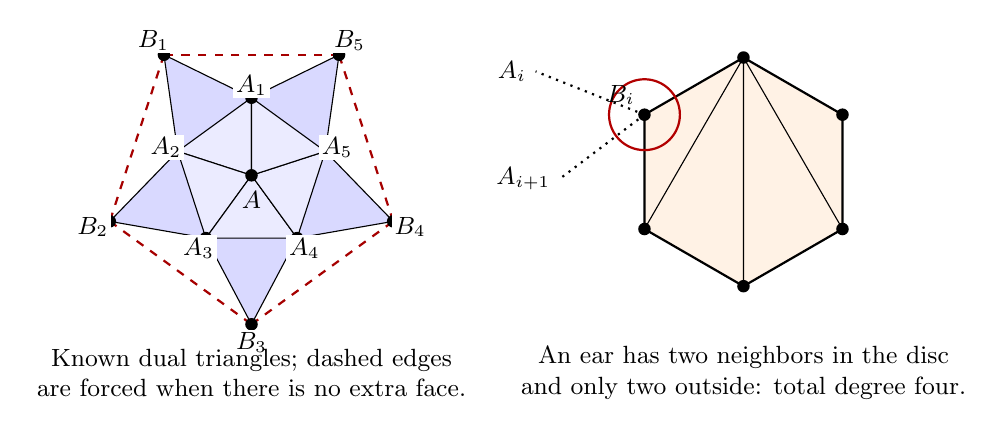
\begin{tikzpicture}[scale=.88,
  dot/.style={circle,fill=black,inner sep=1.6pt},
  every node/.style={font=\small}]
  \begin{scope}[xshift=-3.7cm]
    \coordinate (Z) at (0,0);
    \foreach \i in {1,...,5}{
      \pgfmathsetmacro{\ang}{90+72*(\i-1)}
      \pgfmathsetmacro{\bang}{126+72*(\i-1)}
      \coordinate (A\i) at (\ang:1.12);
      \coordinate (B\i) at (\bang:2.15);
    }
    \foreach \i in {1,...,5}{
      \pgfmathtruncatemacro{\j}{mod(\i,5)+1}
      \fill[blue!8] (Z)--(A\i)--(A\j)--cycle;
      \fill[blue!15] (A\i)--(B\i)--(A\j)--cycle;
      \draw (Z)--(A\i)--(A\j)--cycle;
      \draw (A\i)--(B\i)--(A\j);
      \draw[dashed,thick,red!65!black] (B\i)--(B\j);
    }
    \node[dot,label=below:$A$] at (Z) {};
    \foreach \i in {1,...,5}{
      \node[dot] at (A\i) {};
      \node[dot] at (B\i) {};
      \node[fill=white,inner sep=1pt] at ($(A\i)!-.16!(Z)$) {$A_{\i}$};
      \node[fill=white,inner sep=1pt] at ($(B\i)!-.12!(Z)$) {$B_{\i}$};
    }
    \node[align=center] at (0,-2.85)
      {Known dual triangles; dashed edges\\are forced when there is no extra face.};
  \end{scope}
  \begin{scope}[xshift=3.4cm,yshift=.05cm]
    \foreach \i in {0,...,5}{
      \pgfmathsetmacro{\ang}{90+60*\i}
      \coordinate (P\i) at (\ang:1.65);
    }
    \fill[orange!10] (P0)--(P1)--(P2)--(P3)--(P4)--(P5)--cycle;
    \draw[thick] (P0)--(P1)--(P2)--(P3)--(P4)--(P5)--cycle;
    \draw (P0)--(P2) (P0)--(P3) (P0)--(P4);
    \foreach \i in {0,...,5}{\node[dot] at (P\i) {};}
    \node[draw=red!70!black,circle,minimum size=9mm,thick] at (P1) {};
    \coordinate (U) at (-3.0,1.45);
    \coordinate (V) at (-2.65,-.1);
    \draw[dotted,thick] (P1)--(U) (P1)--(V);
    \node[left] at (U) {$A_i$};
    \node[left] at (V) {$A_{i+1}$};
    \node[above left] at (P1) {$B_i$};
    \node[align=center] at (0,-2.9)
      {An ear has two neighbors in the disc\\and only two outside: total degree four.};
  \end{scope}
\end{tikzpicture}
\caption{The dual closing argument. The left panel depicts the cyclic
incidences for $k=5$; the argument works for every $k\ge5$. The right
panel is a schematic triangulated complementary disc. These are
combinatorial drawings, not metric hyperbolic models.}
\label{fig:ear}
\end{figure}

The equality pattern can be recognized without a small-polyhedron list.
When there is exactly one extra face and it meets none of the $A_i$,
it is the unique interior vertex of the complementary $B$-disc. A chord
between two $B_i$ would cut off a polygon without this interior vertex.
The ear fact, applied away from that chord's endpoints, again gives a
$B_i$ of total degree four. Thus there are no chords and the extra face
joins every $B_i$. The result has two $k$-gons and two cyclic rows of
$k$ pentagons: the L\"obell face lattice. This agrees with the usual
description in~\cite[p.~17 of the author's version]{KK}. We need only
the proved disjointness of the extra face, and do not invoke metric
rigidity of this lattice.

\section{Capacity around a three-dimensional facet}

\begin{proof}[Proof of Theorem~\ref{thm:capacity}]
Let $F$ have $V$ vertices and $M$ two-faces. Trivalence and Euler's
formula inside $F$ give
\begin{equation}\label{eq:M}
 M=V/2+2.
\end{equation}
There are $M$ neighboring facets $F_1,\ldots,F_M$ and $V$ distinct
perpendicular-edge opposites $R_x$. Thus $1+M+V$ facets are already
counted. Call any other facet extra.

Suppose the ridge $F\cap F_i$ has $k_i$ sides. Inside $F_i$, the known
faces are precisely this ridge, its $k_i$ neighbors coming from the
other $F_j$, and its $k_i$ perpendicular-edge opposites coming from the
$R_x$ at its vertices. The perpendicular edges in $F_i$ are the same
edges of $P$ used in Lemma~\ref{lem:opposite}. If a different $F_j$
meets $F_i$, their three pairwise orthogonal normals with that of $F$
give an actual common edge by Lemma~\ref{lem:gap}; hence it is already
one of those $k_i$ neighbors. The opposite-incidence equivalence in
Lemma~\ref{lem:opposite} makes the list of $R_x$ exact as well.

Let $e_i$ count the further faces of $F_i$, all coming from extra
facets of $P$. Lemma~\ref{lem:polygon} gives $e_i\ge1$. An extra facet
has footprint at most two among the $F_j$. Indeed its footprint is a
clique by Lemma~\ref{lem:footprint}. Three members of this clique have
mutually orthogonal normals in the Lorentz space $a^\perp$ of signature
$(3,1)$, where $a$ is the normal of $F$. Together with $a$, they give
an actual vertex $x$ of $F$. A facet meeting all three is $R_x$, already
counted. A larger orthogonal collection cannot fit in $a^\perp$.

There is an additional restriction when $e_i=1$. The equality part of
Lemma~\ref{lem:polygon} says that its unique extra face is disjoint
from all the $k_i$ neighboring faces of $F\cap F_i$ inside $F_i$.
The parent extra facet cannot also meet another $F_j$: such a meeting
would force a common edge with $F_i,F_j$, contradicting that
disjointness. This extra facet therefore has singleton footprint
$\{i\}$.

Let $s$ be the number of indices with $e_i=1$. Their extra facets are
distinct and cannot serve any other index. The other $M-s$ indices
require at least $\sum_{e_i\ge2}e_i$ incidences. Since every remaining
extra facet serves at most two indices, the number of distinct extras
is at least
\[
 s+\frac12\sum_{e_i\ge2}e_i\ \ge\ s+(M-s)=M.
\]
Adding the previously counted facets and using~\eqref{eq:M} proves
\[
 f\ge1+M+V+M=2V+5.
\]
\end{proof}

\begin{figure}[tb]
\centering
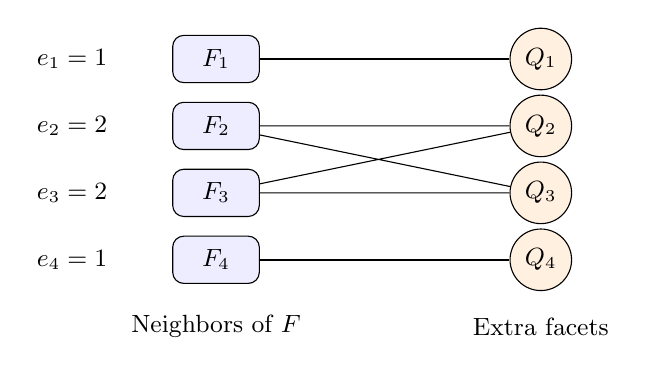
\begin{tikzpicture}[x=2.5cm,y=.85cm,
  face/.style={draw,rounded corners,fill=blue!7,minimum width=11mm,minimum height=6mm},
  extra/.style={draw,circle,fill=orange!12,inner sep=3pt},
  every node/.style={font=\small}]
  \foreach \i/\y in {1/3,2/2,3/1,4/0}{
    \node[face] (F\i) at (0,\y) {$F_{\i}$};
    \node[extra] (Q\i) at (1.65,\y) {$Q_{\i}$};
  }
  \draw[thick] (F1)--(Q1) (F4)--(Q4);
  \draw (F2)--(Q2) (F2)--(Q3) (F3)--(Q2) (F3)--(Q3);
  \node[left=7mm of F1] {$e_1=1$};
  \node[left=7mm of F2] {$e_2=2$};
  \node[left=7mm of F3] {$e_3=2$};
  \node[left=7mm of F4] {$e_4=1$};
  \node[align=center] at (0,-1.0) {Neighbors of $F$};
  \node[align=center] at (1.65,-1.0) {Extra facets};
\end{tikzpicture}
\caption{The final capacity count, shown as an incidence graph rather
than a claimed polytope realization. An index with $e_i=1$ consumes a
distinct singleton. Every other index needs at least two incidences,
while each remaining extra facet can serve at most two indices.}
\label{fig:capacity}
\end{figure}

\section{Pentagon excess and the volume reduction}

Because $P$ is simple, $e=2v$. Euler's formula for its boundary gives
$v-e+r-f=0$, hence $r=v+f$. At each vertex the link is a tetrahedron,
so six ridges meet there. Counting their corners yields
\[
 \sum_R k(R)=6v.
\]
It follows that
\[
 W=6v-5r=v-5f\ge0.
\]
Inside a facet $F$, trivalence gives $2E_F=3V$ and Euler gives
$M=V/2+2$. Therefore
\begin{equation}\label{eq:facet-excess}
 d(F)=3V-5M=\frac{V-20}{2}.
\end{equation}
Each ridge belongs to two facets, so $\sum_Fd(F)=2W$. In particular
$W\ge d(F)$, since all ridge excesses are nonnegative.

For completeness the compact volume formula can be recovered from the
reflection orbifold. The stabilizer of the interior of a codimension-$j$
face is a product of $j$ groups of order two. Its Euler characteristic
is consequently
\[
 \chi_{\mathrm{orb}}
 =1-\frac f2+\frac r4-\frac e8+\frac v{16}
 =\frac{v-4f+16}{16}.
\]
Chern--Gauss--Bonnet in dimension four gives
\[
 \Vol(P)=\frac{4\pi^2}{3}\chi_{\mathrm{orb}}
 =\frac{\pi^2}{12}(v-4f+16)
 =\frac{\pi^2}{12}(f+W+16),
\]
as in~\eqref{eq:volume}.

Combining Theorem~\ref{thm:capacity} with~\eqref{eq:facet-excess} gives
\[
 f+W\ge2V+5+\frac{V-20}{2}=\frac52V-5.
\]
If $\Vol(P)<34\pi^2/3$, then $f+W<120$, so $V<50$.
The integer $V$ is even by trivalence, giving $V\le48$. The non-strict
comparison gives $V\le50$. Likewise the strict double-volume comparison
gives $f+W<256$, whence $V<522/5$ and $V\le104$. This proves
Corollary~\ref{cor:local-size}.

\section{Limits of the argument}

For a dodecahedral facet, Theorem~\ref{thm:capacity} starts at $45$
facets. It does not reach $120$. Nor does it force a polytope containing
a dodecahedral facet to contain a regular $120$-cell. The remaining
possibilities in the strict smaller-volume problem have facets with at
most $48$ vertices, but their mutual geometric compatibility is not
settled by the single-facet count. The same limitation is stronger still
for the proposed second-volume problem.

The proof is a written geometric argument. Its normal, topological and
orbifold interfaces have not been formalized in Lean. No numerical
search or bounded polytope census is used, and no novelty or published
priority claim is attached to the capacity inequality.

\begin{thebibliography}{9}
\bibitem{AVS}
D.~V.~Alekseevskij, E.~B.~Vinberg and A.~S.~Solodovnikov,
\emph{Geometry of spaces of constant curvature}, in
\emph{Geometry II}, Encyclopaedia of Mathematical Sciences~29,
Springer, 1993, pp.~1--138.

\bibitem{PV}
L.~Potyagailo and E.~Vinberg,
\emph{On right-angled reflection groups in hyperbolic spaces},
Commentarii Mathematici Helvetici~80 (2005), 63--73.
\url{https://ems.press/content/serial-article-files/43032}.

\bibitem{KP}
R.~Kellerhals and G.~Perren,
\emph{On the growth of cocompact hyperbolic Coxeter groups},
European Journal of Combinatorics~32 (2011), 1299--1316.

\bibitem{KK}
R.~Kellerhals and A.~Kolpakov,
\emph{The minimal growth rate of cocompact Coxeter groups in hyperbolic
three-space}, Canadian Journal of Mathematics~66 (2014), 354--372.
\url{https://homeweb.unifr.ch/kellerha/pub/CJM-KellKolp-J0844-FINAL.pdf}.
\end{thebibliography}
\end{document}
